% ============================================================================
% CHAPTER 1C: ELECTRICAL SYSTEMS
% ============================================================================

\section{Electrical Systems}
\label{sec:electrical}

Electrical circuits provide clean examples of dynamic systems with well-defined mathematical models. The concepts developed here---impedance, frequency response, filtering---form the historical foundation of control theory.
\begin{historicalbox}[title=Historical Context: Black's Negative Feedback Amplifier and Frequency Response Methods]
The foundation of modern control theory emerged not from mechanical engineers but from electrical engineers at Bell Telephone Laboratories. In 1927, Harold Black invented the negative feedback amplifier, recognizing that feeding a portion of the output back inverted to the input could stabilize amplifier gain against component variations and temperature changes. This elegant insight---that feedback could improve performance---was initially rejected by patent offices, who considered it obvious. Yet Black's feedback amplifier enabled long-distance telephone transmission by compensating for signal loss over cables, fundamentally changing telecommunications.

The mathematical analysis of feedback systems was subsequently developed by Harry Nyquist (1932) and Hendrik Bode (1945), who created graphical methods to analyze stability and performance from frequency response measurements. The Nyquist stability criterion and Bode plots transformed control design from an empirical art into a quantitative science. These frequency response techniques, born from electrical circuits and amplifiers, became universal tools applicable to all domains---mechanical, thermal, biological, and beyond---establishing electrical systems as the historical birthplace of modern control theory.
\end{historicalbox}

% ============================================================================
\subsection{Passive Circuit Elements}
\label{subsec:passive_elements}
% ============================================================================

\subsubsection{Resistor}

Ohm's law relates voltage and current:
\begin{equation}
v(t) = Ri(t)
\end{equation}

In the Laplace domain: $V(s) = RI(s)$

Impedance: $Z_R(s) = R$

\begin{figure}[htbp]
\centering
\begin{circuitikz}[scale=1.2]
    \draw (0,0) to[R, l=$R$, v=$v$, i=$i$] (3,0);
\end{circuitikz}
\caption{Resistor element.}
\label{fig:resistor}
\end{figure}

\subsubsection{Capacitor}

The capacitor stores charge:
\begin{equation}
i(t) = C\frac{\dd v}{\dd t} \quad \Leftrightarrow \quad v(t) = \frac{1}{C}\int i(\tau)\,\dd\tau
\end{equation}

In the Laplace domain: $I(s) = CsV(s)$ or $V(s) = \frac{1}{Cs}I(s)$

Impedance: $Z_C(s) = \frac{1}{Cs}$

\begin{figure}[htbp]
\centering
\begin{circuitikz}[scale=1.2]
    \draw (0,0) to[C, l=$C$, v=$v$, i=$i$] (3,0);
\end{circuitikz}
\caption{Capacitor element.}
\label{fig:capacitor}
\end{figure}

\subsubsection{Inductor}

The inductor stores magnetic energy:
\begin{equation}
v(t) = L\frac{\dd i}{\dd t} \quad \Leftrightarrow \quad i(t) = \frac{1}{L}\int v(\tau)\,\dd\tau
\end{equation}

In the Laplace domain: $V(s) = LsI(s)$ or $I(s) = \frac{1}{Ls}V(s)$

Impedance: $Z_L(s) = Ls$

\begin{figure}[htbp]
\centering
\begin{circuitikz}[scale=1.2]
    \draw (0,0) to[L, l=$L$, v=$v$, i=$i$] (3,0);
\end{circuitikz}
\caption{Inductor element.}
\label{fig:inductor}
\end{figure}

\begin{figure}[htbp]
\centering
\begin{tikzpicture}[scale=1.2]
% Draw axes
\draw[thick, UofSCBlack, ->] (-2, 0) -- (4, 0) node[anchor=west] {Real Axis};
\draw[thick, UofSCBlack, ->] (0, -2.5) -- (0, 3.5) node[anchor=south] {Imaginary Axis};

% Grid and axis labels
\foreach \x in {-2, -1, 0, 1, 2, 3} {
    \draw[UofSC50Black, very thin] (\x, -2.5) -- (\x, 3.5);
    \node[anchor=north] at (\x, -2.5) {\small $\x$};
}
\foreach \y in {-2, -1, 0, 1, 2, 3} {
    \draw[UofSC50Black, very thin] (-2, \y) -- (4, \y);
    \node[anchor=east] at (-2, \y) {\small $\y$};
}

% Resistor: point on real axis
\draw[UofSCGarnet, fill=UofSCGarnet] (2, 0) circle (3pt);
\node[anchor=south, color=UofSCGarnet, font=\small\bfseries] at (2, 0.3) {$R$};

% Inductor: vertical line going up (positive imaginary)
\draw[UofSCAtlantic, thick, ->] (1, 0) -- (1, 2.5);
\node[anchor=west, color=UofSCAtlantic, font=\small\bfseries] at (1.1, 1.3) {$\jj\omega L$};
\draw[UofSCAtlantic, fill=UofSCAtlantic] (1, 2.5) circle (3pt);

% Capacitor: vertical line going down (negative imaginary)
\draw[UofSCHorseshoe, thick, ->] (3, 0) -- (3, -2);
\node[anchor=west, color=UofSCHorseshoe, font=\small\bfseries] at (3.1, -1) {$-\jj/({\omega C})$};
\draw[UofSCHorseshoe, fill=UofSCHorseshoe] (3, -2) circle (3pt);

% Annotations
\node[anchor=north, color=UofSCGarnet, font=\footnotesize] at (2, -0.3) {Pure Resistance};
\node[anchor=south east, color=UofSCAtlantic, font=\footnotesize] at (0.5, 2.7) {Inductive Reactance};
\node[anchor=south east, color=UofSCHorseshoe, font=\footnotesize] at (2.5, -2.2) {Capacitive Reactance};
\end{tikzpicture}
\caption{Impedance in the complex plane showing resistive, inductive, and capacitive elements.}
\label{fig:impedance_plane}
\end{figure}

% ============================================================================
\subsection{RC Circuit (First-Order System)}
\label{subsec:rc_circuit}
% ============================================================================

\begin{figure}[htbp]
\centering
\begin{circuitikz}[scale=1.2]
    \draw (0,0) to[V, l=$v_{\text{in}}$] (0,3)
          to[R, l=$R$, i=$i$] (3,3)
          to[C, l=$C$, v=$v_{\text{out}}$] (3,0)
          -- (0,0);
\end{circuitikz}
\caption{RC low-pass filter circuit.}
\label{fig:rc_circuit}
\end{figure}

\subsubsection{Time-Domain Analysis}

Applying KVL:
\begin{equation}
v_{\text{in}} = v_R + v_{\text{out}} = Ri + v_{\text{out}}
\end{equation}

Since $i = C\frac{\dd v_{\text{out}}}{\dd t}$:
\begin{equation}
\boxed{RC\frac{\dd v_{\text{out}}}{\dd t} + v_{\text{out}} = v_{\text{in}}}
\end{equation}

This is a first-order ODE with time constant $\tau = RC$.

\subsubsection{Transfer Function}

\begin{equation}
G(s) = \frac{V_{\text{out}}(s)}{V_{\text{in}}(s)} = \frac{1}{RCs + 1} = \frac{1}{\tau s + 1}
\end{equation}

\subsubsection{Frequency Response}

Substituting $s = \jj\omega$:
\begin{equation}
G(\jj\omega) = \frac{1}{1 + \jj\omega RC}
\end{equation}

Magnitude and phase:
\begin{align}
|G(\jj\omega)| &= \frac{1}{\sqrt{1 + (\omega RC)^2}} \\
\angle G(\jj\omega) &= -\arctan(\omega RC)
\end{align}

Cutoff frequency (where magnitude is $1/\sqrt{2}$ or $-3$ dB):
\begin{equation}
\omega_c = \frac{1}{RC} = \frac{1}{\tau}
\end{equation}

\begin{examplebox}[title=Example 1.6: RC Circuit Step Response]
An RC circuit has $R = 10$ k$\Omega$ and $C = 1$ $\mu$F. Find:
\begin{enumerate}[label=(\alph*)]
    \item Time constant
    \item Cutoff frequency
    \item Response to a 5V step input
\end{enumerate}

\textbf{Solution:}

(a) Time constant:
\begin{equation}
\tau = RC = 10{,}000 \times 10^{-6} = 0.01 \text{ s} = 10 \text{ ms}
\end{equation}

(b) Cutoff frequency:
\begin{equation}
f_c = \frac{1}{2\pi RC} = \frac{1}{2\pi \times 0.01} = 15.9 \text{ Hz}
\end{equation}

(c) Step response:
\begin{equation}
v_{\text{out}}(t) = 5(1 - \ee^{-t/0.01}) = 5(1 - \ee^{-100t}) \text{ V}
\end{equation}

At $t = \tau = 10$ ms: $v_{\text{out}} = 5(1 - \ee^{-1}) = 3.16$ V (63.2\% of final)
\end{examplebox}

\begin{figure}[htbp]
\centering
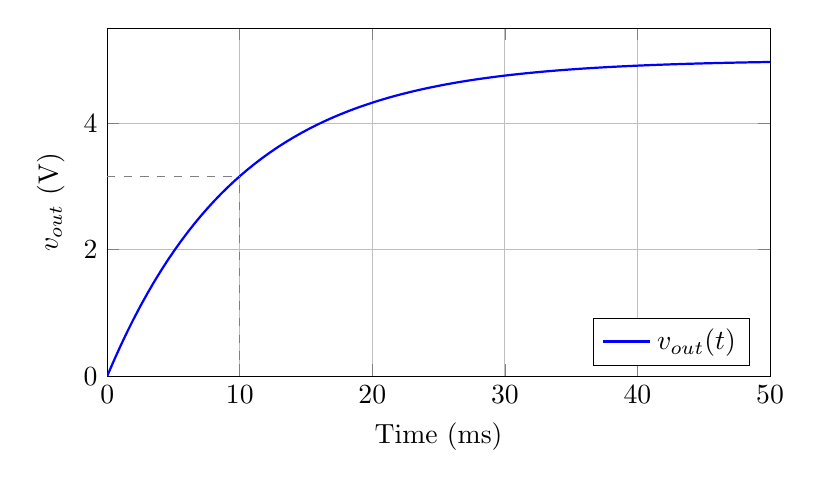
\begin{tikzpicture}
\begin{axis}[
    width=10cm, height=6cm,
    xlabel={Time (ms)},
    ylabel={$v_{\text{out}}$ (V)},
    xmin=0, xmax=50,
    ymin=0, ymax=5.5,
    grid=major,
    legend pos=south east
]
\addplot[blue, thick, domain=0:50, samples=100] {5*(1 - exp(-x/10))};
\addlegendentry{$v_{\text{out}}(t)$}

\draw[dashed, gray] (axis cs:10,0) -- (axis cs:10,3.16);
\draw[dashed, gray] (axis cs:0,3.16) -- (axis cs:10,3.16);
\node[left] at (axis cs:0,3.16) {3.16};
\node[below] at (axis cs:10,0) {$\tau$};
\end{axis}
\end{tikzpicture}
\caption{RC circuit step response.}
\label{fig:rc_step}
\end{figure}

\begin{figure}[htbp]
\centering
\begin{tikzpicture}
\begin{axis}[
    width=10cm, height=5cm,
    xlabel={Frequency (rad/s)},
    ylabel={Magnitude (dB)},
    xmin=0.1, xmax=1000,
    ymin=-60, ymax=5,
    xmode=log,
    grid=major,
    legend pos=south west,
    title={RC Low-Pass Filter: Bode Magnitude Plot ($\omega_c = 100$ rad/s)},
    title style={font=\small, color=UofSCBlack}
]
\addplot[UofSCGarnet, thick, domain=0.1:1000, samples=200] {20*log10(1/sqrt(1 + (x/100)^2))};
\addlegendentry{$|G(\jj\omega)|$}

% Cutoff frequency marker
\draw[dashed, UofSCAtlantic, thick] (axis cs:100,-3) -- (axis cs:100,-65);
\node[anchor=south, color=UofSCAtlantic] at (axis cs:100,-65) {$\omega_c$};
\draw[mark=*, mark size=4pt, mark options={UofSCAtlantic}] plot coordinates {(100, -3)};
\end{axis}
\end{tikzpicture}
\end{figure}

\begin{figure}[htbp]
\centering
\begin{tikzpicture}
\begin{axis}[
    width=10cm, height=5cm,
    xlabel={Frequency (rad/s)},
    ylabel={Phase (degrees)},
    xmin=0.1, xmax=1000,
    ymin=-100, ymax=5,
    xmode=log,
    grid=major,
    legend pos=south west,
    title={RC Low-Pass Filter: Bode Phase Plot},
    title style={font=\small, color=UofSCBlack}
]
\addplot[UofSCAtlantic, thick, domain=0.1:1000, samples=200] {-atan(x/100)*180/pi};
\addlegendentry{$\angle G(\jj\omega)$}

% Cutoff frequency marker (-45°)
\draw[dashed, UofSCHorseshoe, thick] (axis cs:100,-45) -- (axis cs:100,10);
\node[anchor=north, color=UofSCHorseshoe] at (axis cs:100,10) {$-45°$ at $\omega_c$};
\draw[mark=*, mark size=4pt, mark options={UofSCHorseshoe}] plot coordinates {(100, -45)};
\end{axis}
\end{tikzpicture}
\caption{RC low-pass filter Bode plots (magnitude and phase).}
\label{fig:rc_bode}
\end{figure}

% ============================================================================
\subsection{RL Circuit}
\label{subsec:rl_circuit}
% ============================================================================

\begin{figure}[htbp]
\centering
\begin{circuitikz}[scale=1.2]
    \draw (0,0) to[V, l=$v_{\text{in}}$] (0,3)
          to[R, l=$R$] (3,3)
          to[L, l=$L$, v=$v_{\text{out}}$] (3,0)
          -- (0,0);
\end{circuitikz}
\caption{RL circuit.}
\label{fig:rl_circuit}
\end{figure}

For current as output:
\begin{equation}
L\frac{\dd i}{\dd t} + Ri = v_{\text{in}}
\end{equation}

Transfer function (voltage to current):
\begin{equation}
\frac{I(s)}{V_{\text{in}}(s)} = \frac{1}{Ls + R} = \frac{1/R}{(L/R)s + 1}
\end{equation}

Time constant: $\tau = L/R$

% ============================================================================
\subsection{RLC Circuit (Second-Order System)}
\label{subsec:rlc_circuit}
% ============================================================================

\begin{figure}[htbp]
\centering
\begin{circuitikz}[scale=1.2]
    \draw (0,0) to[V, l=$v_{\text{in}}$] (0,4)
          to[R, l=$R$] (2,4)
          to[L, l=$L$] (4,4)
          to[C, l=$C$, v=$v_{\text{out}}$] (4,0)
          -- (0,0);

    % Current direction arrows on the wire
    \draw[->, thick, UofSCAtlantic] (0.2, 4.3) -- (0.8, 4.3) node[above, font=\small, color=UofSCAtlantic] {$i(t)$};
    \draw[->, thick, UofSCAtlantic] (2.2, 4.3) -- (2.8, 4.3);
    \draw[->, thick, UofSCAtlantic] (4.2, 3.5) -- (4.2, 3);

    % Node voltage labels
    \node[above, font=\small, color=UofSCHorseshoe] at (0, 4.3) {$v_{\text{in}}$};
    \node[above, font=\small, color=UofSCHorseshoe] at (2, 4.3) {$v_R$};
    \node[above, font=\small, color=UofSCHorseshoe] at (4, 4.3) {$v_L$};
    \node[right, font=\small, color=UofSCHorseshoe] at (4.3, 2) {$v_C$};
\end{circuitikz}
\caption{Series RLC circuit with current direction and node voltages labeled.}
\label{fig:rlc_circuit}
\end{figure}

\subsubsection{Differential Equation}

Applying KVL:
\begin{equation}
v_{\text{in}} = v_R + v_L + v_C = Ri + L\frac{\dd i}{\dd t} + v_{\text{out}}
\end{equation}

Since $i = C\frac{\dd v_{\text{out}}}{\dd t}$:
\begin{equation}
\boxed{LC\frac{\dd^2 v_{\text{out}}}{\dd t^2} + RC\frac{\dd v_{\text{out}}}{\dd t} + v_{\text{out}} = v_{\text{in}}}
\end{equation}

\subsubsection{Transfer Function}

\begin{equation}
G(s) = \frac{V_{\text{out}}(s)}{V_{\text{in}}(s)} = \frac{1}{LCs^2 + RCs + 1}
\end{equation}

In standard form:
\begin{equation}
G(s) = \frac{\omega_n^2}{s^2 + 2\zeta\omega_n s + \omega_n^2}
\end{equation}

where:
\begin{align}
\omega_n &= \frac{1}{\sqrt{LC}} \quad \text{(resonant frequency)} \\
\zeta &= \frac{R}{2}\sqrt{\frac{C}{L}} \quad \text{(damping ratio)}
\end{align}

\subsubsection{Quality Factor}

The quality factor $Q$ measures the sharpness of resonance:
\begin{equation}
Q = \frac{1}{2\zeta} = \frac{1}{R}\sqrt{\frac{L}{C}}
\end{equation}

High $Q$ means sharp resonance peak and low damping.

\begin{examplebox}[title=Example 1.7: RLC Circuit Design]
Design an RLC circuit with resonant frequency $f_n = 1$ kHz and $Q = 10$.

\textbf{Solution:}

Choose $C = 0.1$ $\mu$F. Then:
\begin{equation}
L = \frac{1}{(2\pi f_n)^2 C} = \frac{1}{(2\pi \times 1000)^2 \times 10^{-7}} = 0.253 \text{ H}
\end{equation}

For $Q = 10$:
\begin{equation}
R = \frac{1}{Q}\sqrt{\frac{L}{C}} = \frac{1}{10}\sqrt{\frac{0.253}{10^{-7}}} = 159 \text{ }\Omega
\end{equation}

Damping ratio: $\zeta = 1/(2Q) = 0.05$ (highly underdamped)
\end{examplebox}

\begin{figure}[htbp]
\centering
\begin{tikzpicture}
\begin{axis}[
    width=12cm, height=6cm,
    xlabel={Frequency (rad/s)},
    ylabel={Magnitude Response $|G(\jj\omega)|$},
    xmin=500, xmax=1500,
    ymin=0, ymax=1.2,
    grid=major,
    legend pos=north east,
    title={RLC Series Circuit Frequency Response ($f_n = 1$ kHz, $Q = 10$)},
    title style={font=\small, color=UofSCBlack}
]

% RLC response with Q=10
\addplot[UofSCGarnet, thick, domain=500:1500, samples=300] {(2*3.14159*1000)^2 / sqrt(((2*3.14159*x)^2 - (2*3.14159*1000)^2)^2 + (2*3.14159*1000*2*3.14159*x/10)^2)};
\addlegendentry{RLC Response ($Q=10$)}

% Resonant frequency marker
\draw[dashed, UofSCAtlantic, thick] (axis cs:6283, 0) -- (axis cs:6283, 1.15);
\draw[mark=*, mark size=5pt, mark options={UofSCAtlantic}] plot coordinates {(6283, 1.05)};
\node[anchor=south, color=UofSCAtlantic, font=\footnotesize] at (axis cs:6283, 1.15) {$\omega_n$};

% Bandwidth markers (-3dB points approx at 0.707 of peak)
\draw[dashed, UofSCHorseshoe] (axis cs:5970, 0.74) -- (axis cs:5970, 0);
\draw[dashed, UofSCHorseshoe] (axis cs:6596, 0.74) -- (axis cs:6596, 0);
\draw[<->, UofSCHorseshoe, thick] (axis cs:5970, -0.08) -- (axis cs:6596, -0.08);
\node[anchor=north, color=UofSCHorseshoe, font=\footnotesize] at (axis cs:6283, -0.15) {BW};

\end{axis}
\end{tikzpicture}
\caption{RLC series circuit frequency response showing resonance peak at $\omega_n$ and bandwidth.}
\label{fig:rlc_frequency_response}
\end{figure}

% ============================================================================
\subsection{Operational Amplifier Circuits}
\label{subsec:opamp}
% ============================================================================

Operational amplifiers (op-amps) are fundamental building blocks for analog control systems.

\subsubsection{Ideal Op-Amp Assumptions}

\begin{itemize}
    \item Infinite open-loop gain: $A \to \infty$
    \item Infinite input impedance: $Z_{\text{in}} \to \infty$ (no input current)
    \item Zero output impedance: $Z_{\text{out}} = 0$
    \item Infinite bandwidth
\end{itemize}

With negative feedback, these lead to the ``golden rules'':
\begin{enumerate}
    \item $V_+ = V_-$ (virtual short)
    \item $I_+ = I_- = 0$ (no input current)
\end{enumerate}

\begin{figure}[htbp]
\centering
\begin{circuitikz}[scale=1.2]
    \draw (0,0) node[op amp] (opamp) {}
    (opamp.+) node[left] {$V_+$}
    (opamp.-) node[left] {$V_-$}
    (opamp.out) node[right] {$V_{\text{out}}$};
\end{circuitikz}
\caption{Op-amp symbol.}
\label{fig:opamp_symbol}
\end{figure}

\subsubsection{Inverting Amplifier}

\begin{figure}[htbp]
\centering
\begin{circuitikz}[scale=1]
    \draw (0,0) node[op amp] (opamp) {};
    \draw (opamp.+) -- ++(-0.5,0) node[ground] {};
    \draw (opamp.-) -- ++(-0.5,0) coordinate (A)
          to[R, l=$R_1$] ++(-2,0) node[left] {$V_{\text{in}}$};
    \draw (A) -- ++(0,1.5) coordinate (B)
          to[R, l=$R_2$] ++(2.5,0) coordinate (C)
          -- (C |- opamp.out) -- (opamp.out);
    \draw (opamp.out) -- ++(0.5,0) node[right] {$V_{\text{out}}$};
\end{circuitikz}
\caption{Inverting amplifier.}
\label{fig:inverting_amp}
\end{figure}

Transfer function:
\begin{equation}
\frac{V_{\text{out}}}{V_{\text{in}}} = -\frac{R_2}{R_1}
\end{equation}

\subsubsection{Non-Inverting Amplifier}

Transfer function:
\begin{equation}
\frac{V_{\text{out}}}{V_{\text{in}}} = 1 + \frac{R_2}{R_1}
\end{equation}

\subsubsection{Integrator}

\begin{figure}[htbp]
\centering
\begin{circuitikz}[scale=1]
    \draw (0,0) node[op amp] (opamp) {};
    \draw (opamp.+) -- ++(-0.5,0) node[ground] {};
    \draw (opamp.-) -- ++(-0.5,0) coordinate (A)
          to[R, l=$R$] ++(-2,0) node[left] {$V_{\text{in}}$};
    \draw (A) -- ++(0,1.5) coordinate (B)
          to[C, l=$C$] ++(2.5,0) coordinate (C)
          -- (C |- opamp.out) -- (opamp.out);
    \draw (opamp.out) -- ++(0.5,0) node[right] {$V_{\text{out}}$};
\end{circuitikz}
\caption{Op-amp integrator.}
\label{fig:integrator}
\end{figure}

Transfer function:
\begin{equation}
G(s) = \frac{V_{\text{out}}(s)}{V_{\text{in}}(s)} = -\frac{1}{RCs}
\end{equation}

Time-domain:
\begin{equation}
v_{\text{out}}(t) = -\frac{1}{RC}\int_0^t v_{\text{in}}(\tau)\,\dd\tau
\end{equation}

\subsubsection{Differentiator}

Transfer function:
\begin{equation}
G(s) = \frac{V_{\text{out}}(s)}{V_{\text{in}}(s)} = -RCs
\end{equation}

\begin{warningbox}
Pure differentiators amplify high-frequency noise. In practice, add a small resistor in series with $C$ to limit high-frequency gain.
\end{warningbox}

\subsubsection{PID Controller Implementation}

A PID controller can be implemented with op-amps:

\begin{equation}
G_{PID}(s) = K_p + \frac{K_i}{s} + K_d s
\end{equation}

\begin{figure}[htbp]
\centering
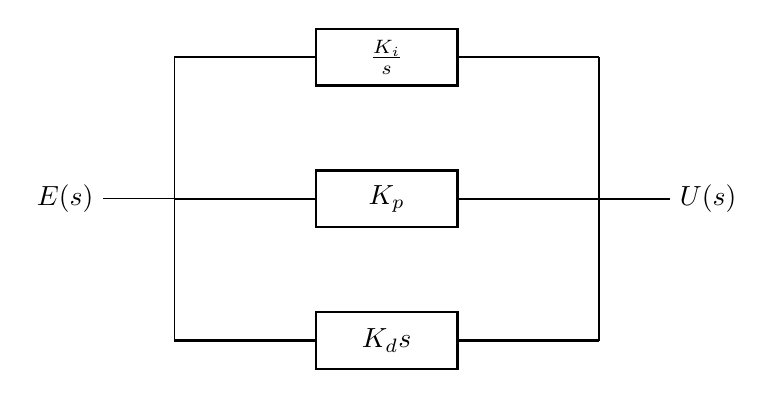
\begin{tikzpicture}[scale=0.9]
    % Input
    \node[left] at (-1,0) {$E(s)$};

    % Summing junction
    \draw[-] (-1,0) -- (0,0);

    % Three parallel paths
    \draw[-] (0,0) -- (0,2);
    \draw[-] (0,0) -- (0,-2);

    % P path
    \draw[thick] (0,0) -- (2,0);
    \draw[thick, fill=white] (2,-0.4) rectangle (4,0.4);
    \node at (3,0) {$K_p$};
    \draw[thick] (4,0) -- (6,0);

    % I path
    \draw[thick] (0,2) -- (2,2);
    \draw[thick, fill=white] (2,1.6) rectangle (4,2.4);
    \node at (3,2) {$\frac{K_i}{s}$};
    \draw[thick] (4,2) -- (6,2);

    % D path
    \draw[thick] (0,-2) -- (2,-2);
    \draw[thick, fill=white] (2,-2.4) rectangle (4,-1.6);
    \node at (3,-2) {$K_d s$};
    \draw[thick] (4,-2) -- (6,-2);

    % Summing
    \draw[thick] (6,2) -- (6,0);
    \draw[thick] (6,-2) -- (6,0);
    \draw[thick] (6,0) -- (7,0);

    % Output
    \node[right] at (7,0) {$U(s)$};
\end{tikzpicture}
\caption{PID controller block diagram.}
\label{fig:pid_block}
\end{figure}

% ============================================================================
\subsection{Active Filters}
\label{subsec:active_filters}
% ============================================================================

\subsubsection{First-Order Low-Pass Filter}

\begin{equation}
G(s) = \frac{K}{s/\omega_c + 1}
\end{equation}

Passes low frequencies, attenuates high frequencies.

\subsubsection{First-Order High-Pass Filter}

\begin{equation}
G(s) = \frac{Ks/\omega_c}{s/\omega_c + 1}
\end{equation}

Passes high frequencies, attenuates low frequencies (including DC).

\subsubsection{Second-Order Butterworth Low-Pass}

Maximally flat passband response:
\begin{equation}
G(s) = \frac{\omega_c^2}{s^2 + \sqrt{2}\omega_c s + \omega_c^2}
\end{equation}

Damping ratio $\zeta = 1/\sqrt{2} \approx 0.707$, giving no overshoot in step response.

\subsubsection{Band-Pass Filter}

\begin{equation}
G(s) = \frac{K(\omega_0/Q)s}{s^2 + (\omega_0/Q)s + \omega_0^2}
\end{equation}

Passes frequencies near $\omega_0$, attenuates both lower and higher frequencies.

\begin{figure}[htbp]
\centering
\begin{tikzpicture}
\begin{axis}[
    width=13cm, height=6.5cm,
    xlabel={Frequency (rad/s)},
    ylabel={Magnitude (dB)},
    xmin=0.1, xmax=10000,
    ymin=-80, ymax=5,
    xmode=log,
    grid=major,
    legend pos=south left,
    legend style={font=\footnotesize},
    title={Filter Type Comparison: Magnitude Response (Normalized Cutoff $\omega_c = 100$ rad/s)},
    title style={font=\small, color=UofSCBlack}
]

% Low-pass filter
\addplot[UofSCGarnet, thick, domain=0.1:10000, samples=200] {20*log10(1/sqrt(1 + (x/100)^2))};
\addlegendentry{Low-Pass}

% High-pass filter
\addplot[UofSCAtlantic, thick, domain=0.1:10000, samples=200] {20*log10((x/100)/sqrt(1 + (x/100)^2))};
\addlegendentry{High-Pass}

% Band-pass filter (Q=5, centered at 100 rad/s)
\addplot[UofSCHorseshoe, thick, domain=0.1:10000, samples=200] {20*log10((x/100)/sqrt((1-(x/100)^2)^2 + (x/(100*5))^2))};
\addlegendentry{Band-Pass}

% Cutoff frequency marker
\draw[dashed, UofSC50Black, thin] (axis cs:100, -80) -- (axis cs:100, 5);
\node[anchor=north, color=UofSC50Black, font=\footnotesize] at (axis cs:100, -80) {$\omega_c$};

\end{axis}
\end{tikzpicture}
\caption{Comparison of filter types showing magnitude response of low-pass, high-pass, and band-pass filters with normalized cutoff frequency.}
\label{fig:filter_comparison}
\end{figure}

% ============================================================================
\subsection{Power Electronics}
\label{subsec:power_electronics}
% ============================================================================

\subsubsection{Buck Converter (Step-Down)}

\begin{figure}[htbp]
\centering
\begin{circuitikz}[scale=0.9]
    \draw (0,0) to[V, l=$V_{\text{in}}$] (0,3)
          to[switch, l=$S$] (2,3)
          to[L, l=$L$] (4,3)
          -- (4,3) to[C, l=$C$] (4,0)
          -- (0,0);
    \draw (2,3) to[D, l=$D$] (2,0);
    \draw (4,3) -- (5,3) to[R, l=$R_L$] (5,0) -- (4,0);
    \draw (5,3) -- (6,3) node[right] {$V_{\text{out}}$};
    \draw (5,0) -- (6,0) node[right] {};
\end{circuitikz}
\caption{Buck converter circuit.}
\label{fig:buck}
\end{figure}

Steady-state output (ideal):
\begin{equation}
V_{\text{out}} = D \cdot V_{\text{in}}
\end{equation}

where $D$ is the duty cycle ($0 \leq D \leq 1$).

Small-signal transfer function (control to output):
\begin{equation}
\frac{\hat{v}_{\text{out}}(s)}{\hat{d}(s)} = V_{\text{in}} \cdot \frac{1}{LCs^2 + (L/R_L)s + 1}
\end{equation}

% ============================================================================
\subsection{Exercises: Electrical Systems}
% ============================================================================

\begin{exercise}
For an RC circuit with $R = 47$ k$\Omega$ and $C = 0.22$ $\mu$F:
\begin{enumerate}[label=(\alph*)]
    \item Find the time constant and cutoff frequency
    \item Sketch the Bode plot (magnitude and phase)
    \item Find the output voltage 5 ms after a 10V step input
\end{enumerate}
\end{exercise}

\begin{exercise}
Design an RLC band-pass filter with center frequency 10 kHz and bandwidth 1 kHz. Calculate $R$, $L$, $C$, and $Q$.
\end{exercise}

\begin{exercise}
An op-amp integrator has $R = 100$ k$\Omega$ and $C = 1$ $\mu$F. If the input is $v_{\text{in}}(t) = 2\sin(100t)$ V:
\begin{enumerate}[label=(\alph*)]
    \item Find the transfer function
    \item Calculate the steady-state output amplitude and phase
    \item Write the time-domain output expression
\end{enumerate}
\end{exercise}

\begin{exercise}
For the series RLC circuit, find the current $i(t)$ response to a unit step voltage input when $R = 100$ $\Omega$, $L = 0.1$ H, and $C = 100$ $\mu$F. Is the circuit underdamped, critically damped, or overdamped?
\end{exercise}

\begin{exercise}
Design a second-order Sallen-Key low-pass filter with cutoff frequency 1 kHz and Butterworth response. Specify all component values.
\end{exercise}

\begin{exercise}
\textbf{Concept:} Compare the frequency response characteristics of three filters:
\begin{enumerate}[label=(\alph*)]
    \item A first-order low-pass filter with $\omega_c = 1000$ rad/s
    \item A second-order Butterworth low-pass filter with $\omega_c = 1000$ rad/s
    \item A first-order high-pass filter with $\omega_c = 1000$ rad/s
\end{enumerate}

For each, sketch the Bode magnitude plot and describe:
\begin{enumerate}[label=(\alph*)]
    \item The slope (dB/decade) in the stopband
    \item The phase shift at the cutoff frequency
    \item Which frequencies are attenuated and which are passed
\end{enumerate}
\end{exercise}

\begin{exercise}
A boost converter steps up a 12V input to 48V at a switching frequency of 200 kHz. Assume efficiency $\eta = 0.92$.

\begin{enumerate}[label=(\alph*)]
    \item Calculate the required duty cycle
    \item If the load draws 5A at 48V, find the input current
    \item Design the filter inductance to limit current ripple to $\pm 5\%$
\end{enumerate}
\end{exercise}

\begin{exercise}
\textbf{Design:} An active low-pass filter must attenuate 60 Hz power line noise by at least 40 dB while preserving signals below 50 Hz.

\begin{enumerate}[label=(\alph*)]
    \item Determine the minimum filter order required
    \item Choose between Butterworth, Chebyshev, and Bessel responses and justify your choice
    \item If using a second-order topology, calculate the component values for unity-gain implementation
    \item Estimate the phase lag at 20 Hz
\end{enumerate}
\end{exercise}

\begin{exercise}
\textbf{Computational:} For the series RLC circuit with $R = 10$ $\Omega$, $L = 1$ H, and $C = 1$ $\mu$F:

\begin{enumerate}[label=(\alph*)]
    \item Find the resonant frequency
    \item Calculate the quality factor $Q$
    \item Find the magnitude of impedance at resonance, at $\omega = \omega_n/2$, and at $2\omega_n$
    \item If driven by $v_{\text{in}}(t) = 100\sin(\omega_n t)$ V, find the steady-state current amplitude at resonance
\end{enumerate}
\end{exercise}

\begin{exercise}
\textbf{Concept:} The PID controller can be implemented using three op-amp stages (one proportional, one integrator, one differentiator).

\begin{enumerate}[label=(\alph*)]
    \item Draw a block diagram showing how three op-amp circuits combine to form a PID controller
    \item Explain the role of each stage in controlling a second-order system
    \item Discuss practical issues with the differentiator stage (e.g., noise) and propose solutions
\end{enumerate}
\end{exercise}
